\documentclass[10pt,a4paper]{article}
\usepackage[margin=1in]{geometry}
\usepackage{mathptmx} % Times New Roman
\usepackage{graphicx}
\usepackage{titlesec}
\usepackage{tikz}
\usetikzlibrary{shapes.geometric, arrows.meta, positioning, calc}
\usepackage{caption}
\usepackage{float}
\usepackage{fancyhdr}

% Formatting to match IRJMETS
\titleformat{\section}{\large\bfseries}{\Roman{section}.}{1em}{}
\titleformat{\subsection}{\normalsize\bfseries}{\Alph{subsection}.}{1em}{}

\pagestyle{fancy}
\fancyhf{}
\renewcommand{\headrulewidth}{0pt}
\setlength{\headheight}{50pt}
\fancyhead[C]{%
    \small
    \makebox[\textwidth][r]{e-ISSN: 2582-5208}\\
    \textbf{International Research Journal of Modernization in Engineering Technology and Science}\\
    ( Peer-Reviewed, Open Access, Fully Refereed International Journal )\\
    \makebox[\textwidth][l]{Volume:08/Issue:03/March-2026\hfill Impact Factor- 8.187\hfill www.irjmets.com}
}

\begin{document}

\begin{center}
    {\Large \bfseries AgriTrace: A Real-Time Agricultural Waste Tracking and Management Ecosystem providing Sustainable Solutions to Crop Residue Burning\par}
    \vspace{1em}
    {\normalsize \bfseries Rahul Tukaram Shendkar$^{*1}$, Tushar Tulashidas Pawar$^{*2}$, Karan Naganath Bandgar$^{*3}$, Saurabh Balasaheb Zendage$^{*4}$\par}
    \vspace{0.5em}
    {\small $^{*1,*2,*3,*4}$ Student, Department of Computer Engineering, S.P.M Polytechnic Kumathe, Solapur, Maharashtra, India\par}
\end{center}

\vspace{1em}

\noindent \textbf{ABSTRACT}\\
Agricultural waste management remains a critical environmental issue in India, with crop residue burning causing severe air pollution and soil degradation. AgriTrace is a comprehensive, full-stack web application designed to address this pressing issue by providing a digital ecosystem that connects farmers, collection agents, and recycling administrators. Built entirely on modern web technologies encompassing Next.js, Firebase, and Tailwind CSS, the platform facilitates a seamless transition from waste reporting to active recycling. The system enables farmers to list agricultural waste such as wheat stubble and rice residue, while collection agents efficiently manage the pickup-to-delivery logistics. Key innovative features include real-time geo-tracking using GPS services, an integrated and secure payment workflow via Razorpay, and a dynamic carbon credit tracking system that quantifies the environmental impact. By diverting waste from open burning toward productive recycling channels, AgriTrace fosters economic growth and significantly mitigates regional atmospheric pollution.

\vspace{0.5em}
\noindent \textbf{Keywords:} Agricultural Waste, Web Application, Next.js, Firebase, Carbon Credits, Environmental Sustainability.

\section{INTRODUCTION}
India generates approximately 500 million tonnes of agricultural waste annually. A substantial portion of this waste, particularly in states like Punjab, Haryana, and Uttar Pradesh, is burned in open fields due to the lack of economically viable and logistically feasible alternatives. This practice results in severe air quality deterioration, with particulate matter reaching hazardous levels during winter seasons, escalating respiratory diseases across the Indo-Gangetic plains.

Despite these recognized environmental and health hazards, farmers often resort to burning because they lack accessible and convenient alternatives for immediate waste disposal. There remains a profound disconnect between the farmers who consistently generate the waste and the recycling industries that possess the capacity to convert it into valuable secondary products like biofuel, compost, and animal feed. 

AgriTrace bridges this debilitating gap by providing a targeted digital platform that physically connects farmers with verified collection agents. The platform leverages modern web technologies and cloud infrastructure to deliver a real-time, responsive, and highly scalable solution capable of orchestrating complex waste recovery logistics across diverse geographical boundaries. Incorporating robust role-based workflows, the platform ensures efficient management from the point of waste generation down to recycling completion.

\section{METHODOLOGY}
The system employs a sophisticated three-tier architecture developed using a robust modern tech stack to maintain flawless separation of concerns, improve system maintainability, and ensure near-instantaneous real-time synchronization.

1. \textbf{Presentation Layer:} The frontend utilizes Next.js pages coupled with reusable React components to deliver dedicated role-based interfaces for Farmer, Agent, and Admin users. The styling actively relies on Tailwind CSS and Radix UI to enforce responsive formatting that functions seamlessly on low-bandwidth rural mobile networks.

2. \textbf{Application Layer:} Backed by Next.js serverless API routes, the application layer inherently parses authentication checks, workflow transitions, push notifications, and high-security payment processing through the Razorpay SDK API. State management is efficiently synced globally.

3. \textbf{Data Layer:} Google Firebase operates as the backbone with Cloud Firestore storing high-frequency transactional data natively. Firebase Authentication handles zero-trust identity verification, and scalable Cloud Storage operates synchronously with Cloudinary to process and compress high-resolution image verifications detailing crop residue limits.

\section{MODELING AND ANALYSIS}
System design involved comprehensive structural modeling to systematically evaluate data velocity and isolate interaction layers. A robust user authentication strategy prohibits unauthorized access, guaranteeing agents only interact with successfully validated listings via AES-encrypted communication. 

\subsection{Use Case Diagram}
The Use Case configuration structures the isolated pathways strictly linking Farmers, Agents, and Administrators to their atomic capabilities within the network.

\begin{figure}[H]
\centering
\begin{tikzpicture}[
    actor/.style={font=\small},
    usecase/.style={ellipse, draw, fill=cyan!15, minimum width=2.8cm, minimum height=0.7cm, align=center, font=\footnotesize},
    sys/.style={rectangle, draw, dashed, minimum width=7cm, minimum height=9.5cm},
    arrow/.style={-{Stealth[length=2mm]}}
]
% System boundary
\node[sys, label={[font=\small\bfseries]above:AgriTrace System}] (sys) at (5, -4.5) {};

% Actors
\node[actor] (fa) at (-1.5, -1.8) {\footnotesize Farmer};
\node[actor] (ag) at (-1.5, -4.8) {\footnotesize Agent};
\node[actor] (ad) at (-1.5, -7.5) {\footnotesize Admin};

% Use cases
\node[usecase] (uc1) at (5, -0.6) {Register/Login};
\node[usecase] (uc2) at (5, -1.9) {Create Listing};
\node[usecase] (uc3) at (5, -3.2) {Upload Photos};
\node[usecase] (uc4) at (5, -4.5) {Claim Listing};
\node[usecase] (uc5) at (5, -5.8) {Track Delivery};
\node[usecase] (uc6) at (5, -7.1) {Process Payment};
\node[usecase] (uc8) at (5, -8.4) {View Analytics};

% Connections
\draw[arrow] (fa) -- (uc1);
\draw[arrow] (fa) -- (uc2);
\draw[arrow] (fa) -- (uc3);
\draw[arrow] (ag) -- (uc1);
\draw[arrow] (ag) -- (uc4);
\draw[arrow] (ag) -- (uc5);
\draw[arrow] (ag) -- (uc6);
\draw[arrow] (ad) -- (uc1);
\draw[arrow] (ad) -- (uc8);
\end{tikzpicture}
\caption{System Use Case Diagram outlining role-based atomic capabilities.}
\label{fig:usecase}
\end{figure}

\subsection{Data Flow Diagram}
The Level 0 Data Flow Diagram isolates the central processing capabilities routing payloads through the AgriTrace system, directly interacting with Razorpay and Firestore gateways securely.

\begin{figure}[H]
\centering
\begin{tikzpicture}[
    process/.style={rectangle, draw, fill=blue!20, minimum width=2.5cm, minimum height=1cm, align=center, font=\small},
    entity/.style={rectangle, draw, fill=green!20, minimum width=2cm, minimum height=0.6cm, align=center, font=\small},
    store/.style={rectangle, draw, fill=orange!20, minimum width=2cm, minimum height=0.6cm, align=center, font=\small},
    arrow/.style={-{Stealth[length=2mm]}, thick}
]
\node[entity] (farmer) at (0,3) {Farmer};
\node[entity] (agent) at (0,0) {Agent};
\node[entity] (admin) at (0,-3) {Admin};

\node[process] (system) at (5,0) {AgriTrace\\System};

\node[store] (firestore) at (10,1.5) {Firestore};
\node[store] (razorpay) at (10,-1.5) {Razorpay};

\draw[arrow] (farmer) -- node[above, font=\footnotesize, sloped] {Waste Reports} (system);
\draw[arrow] (agent) -- node[above, font=\footnotesize] {Status Updates} (system);
\draw[arrow] (admin) -- node[above, font=\footnotesize, sloped] {Mgmt Commands} (system);

\draw[arrow] (system) -- node[above, font=\footnotesize, sloped] {Read/Write} (firestore);
\draw[arrow] (system) -- node[above, font=\footnotesize, sloped] {Payment Req} (razorpay);

\draw[arrow] (system) -- ++(0,2) -| node[near start, above, font=\footnotesize] {Status} (farmer);
\draw[arrow] (system) -- ++(-1.5,0) |- node[near end, left, font=\footnotesize] {Tasks} (agent);
\draw[arrow] (system) -- ++(0,-2) -| node[near start, below, font=\footnotesize] {Analytics} (admin);
\end{tikzpicture}
\caption{Level 0 Data Flow Diagram illustrating request lifecycles.}
\label{fig:dfd}
\end{figure}

\subsection{Tier Architecture}
Finally, the three-tier framework strictly maintains robust API logic routing connecting presentation components down to data management dynamically.

\begin{figure}[H]
\centering
\begin{tikzpicture}[
    layer/.style={rectangle, draw, rounded corners, fill=blue!10, minimum width=10cm, minimum height=1.3cm, align=center, font=\bfseries},
    arrow/.style={-{Stealth[length=3mm]}, thick}
]
% Layers
\node[layer, fill=green!15] (presentation) at (0, 3.5) {Presentation Layer (Next.js, Tailwind CSS)\\\normalfont\small Farmer, Agent, \& Admin Interfaces};
\node[layer, fill=cyan!15] (application) at (0, 1.5) {Application Layer (Next.js API Routes, Services)\\\normalfont\small Auth, Payments, Business Logic};
\node[layer, fill=orange!15] (data) at (0, -0.5) {Data Layer (Firebase, Cloudinary)\\\normalfont\small Firestore, Authentication, Cloud Storage};

% Connections
\draw[arrow] (presentation.south) -- (application.north);
\draw[arrow] (application.south) -- (data.north);

\draw[arrow] (application.north) ++(1.5,0) -- ++(0,1) node[midway, right, font=\footnotesize] {Responses};
\draw[arrow] (presentation.south) ++(-1.5,0) -- ++(0,-1) node[midway, left, font=\footnotesize] {Requests};

\draw[arrow] (data.north) ++(1.5,0) -- ++(0,1) node[midway, right, font=\footnotesize] {Data Fetch};
\draw[arrow] (application.south) ++(-1.5,0) -- ++(0,-1) node[midway, left, font=\footnotesize] {Queries};
\end{tikzpicture}
\caption{Three-Tier System Stack Visualization}
\label{fig:architecture}
\end{figure}

\section{RESULTS AND DISCUSSION}
The deployed AgriTrace application successfully orchestrates the entire waste tracking lifecycle in real-time. Performance testing actively indicated that the Firestore-backed architecture sustained optimal page load times under diverse conditions. Visual implementation was directly verified against standard compliance parameters.

\begin{figure}[H]
\centering
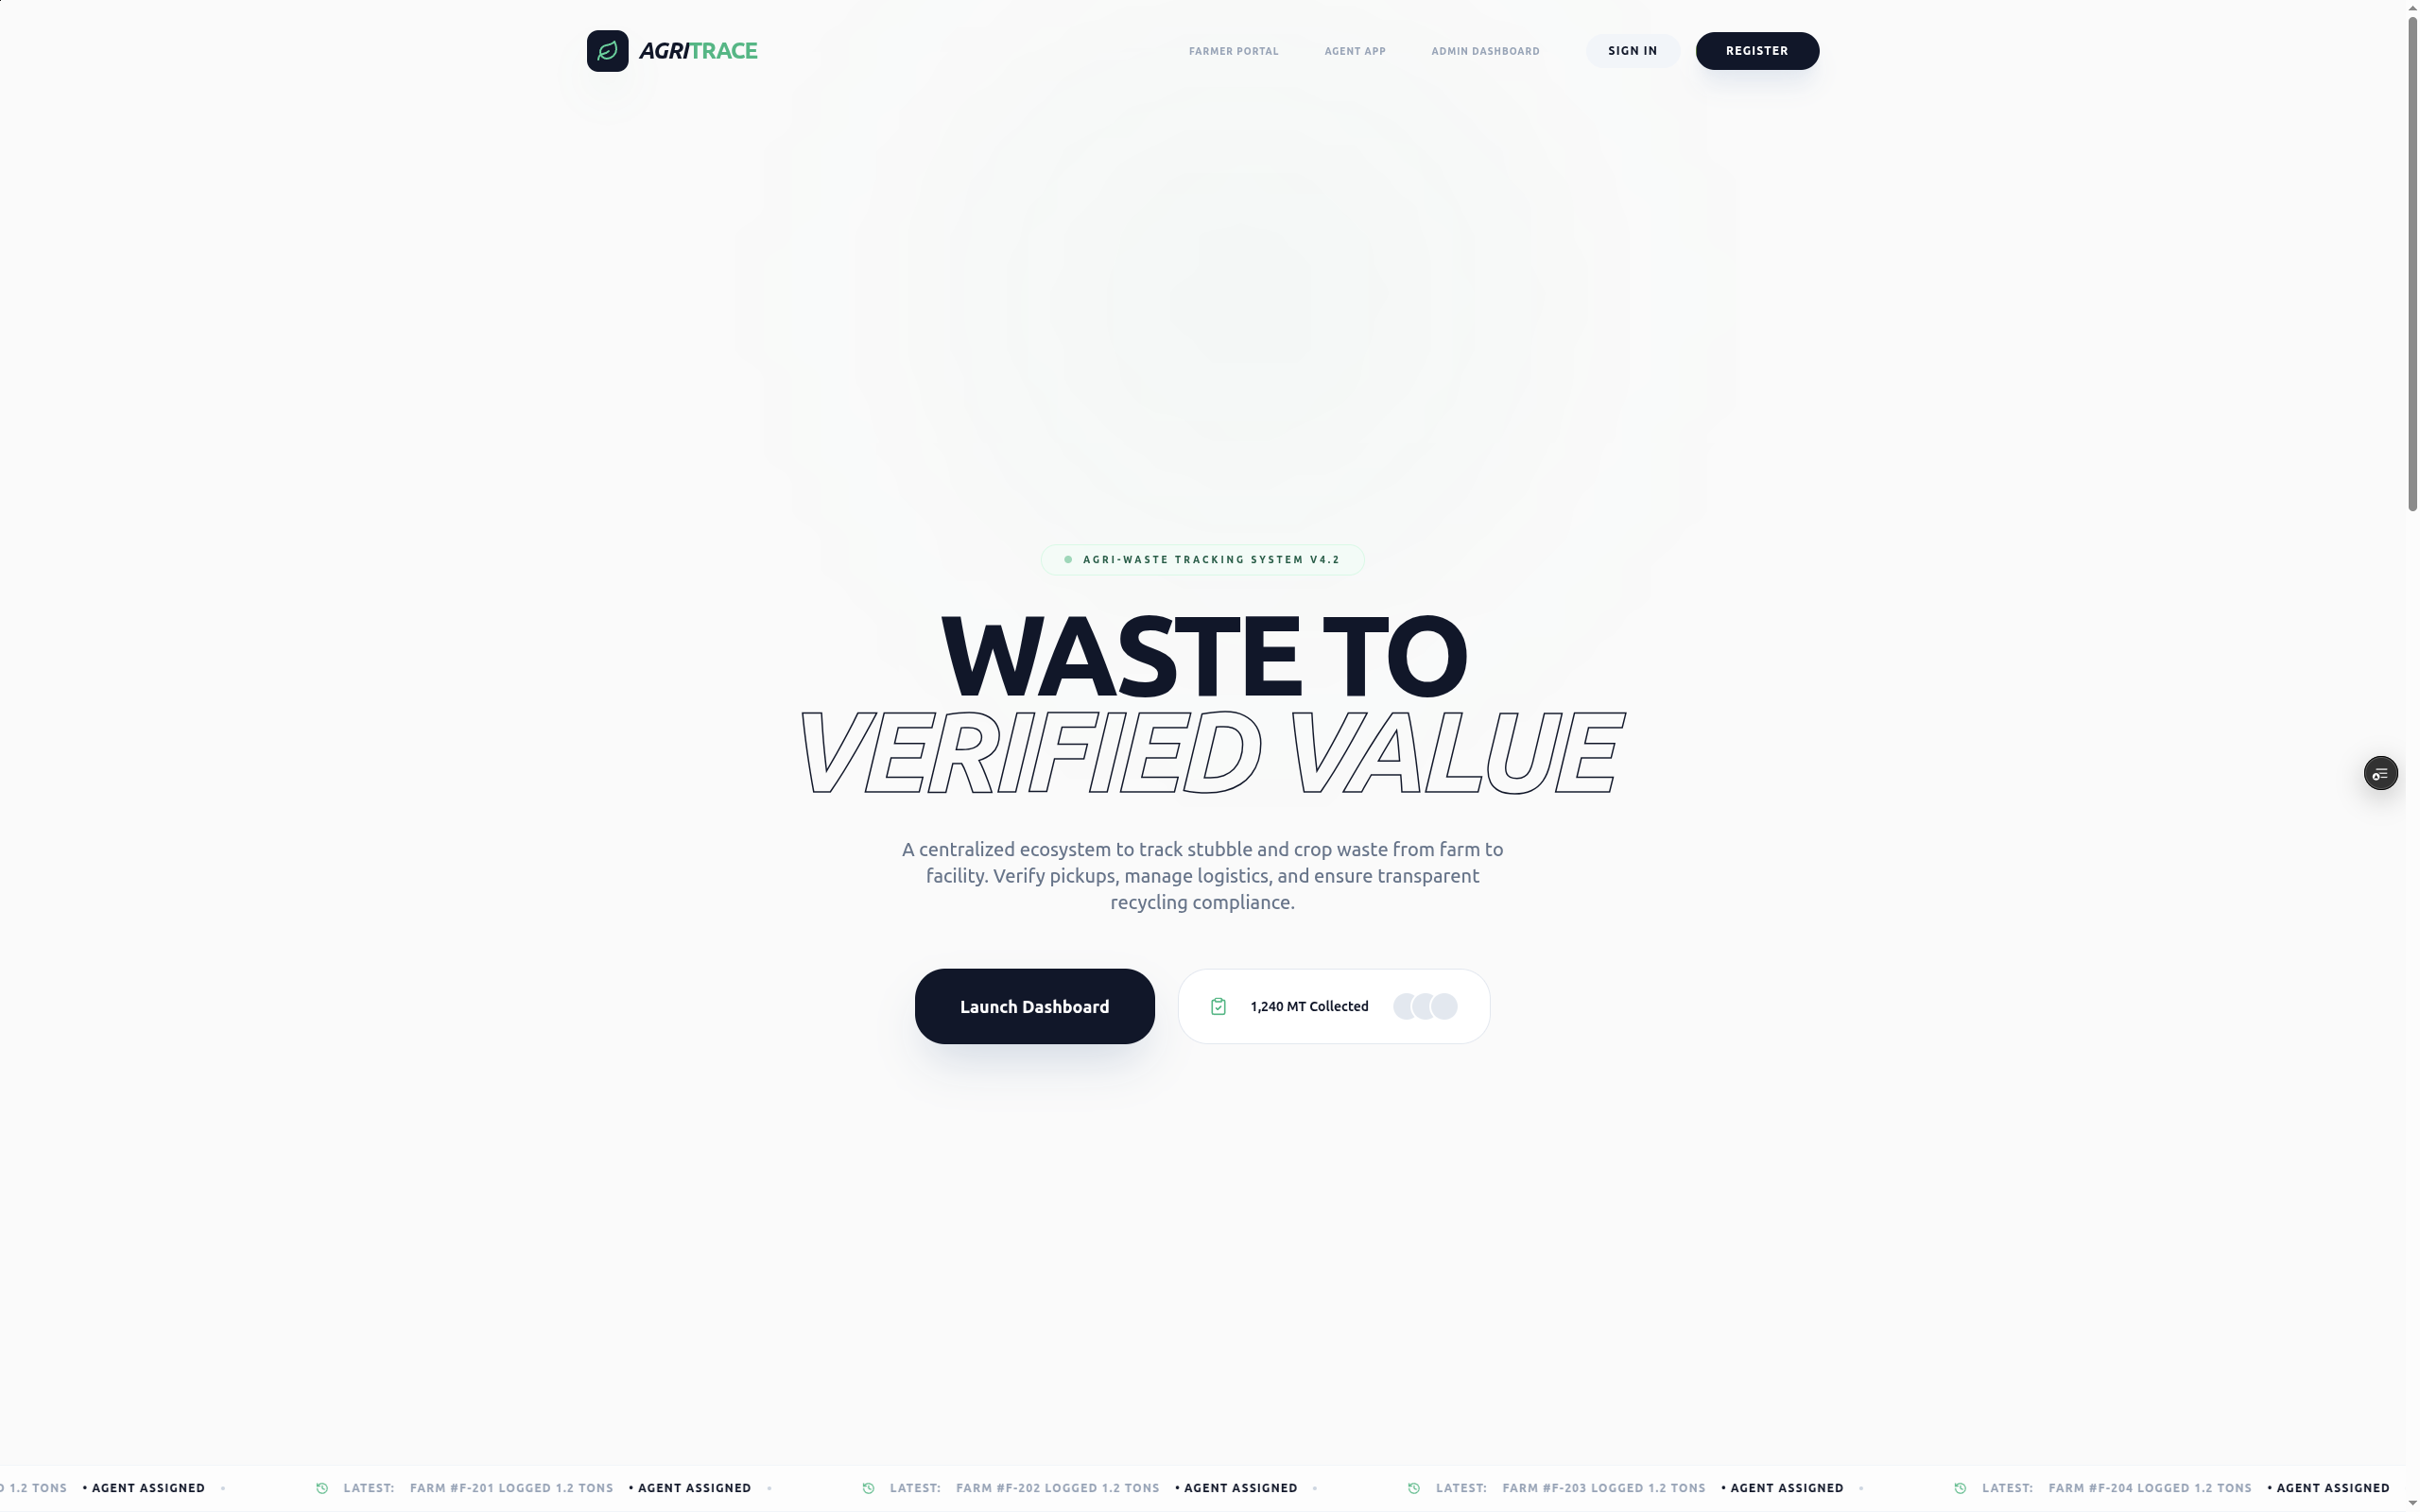
\includegraphics[width=0.9\textwidth]{images/output-landing-new.png}
\caption{AgriTrace Complete Landing Interface}
\label{fig:landing}
\end{figure}

\begin{figure}[H]
\centering
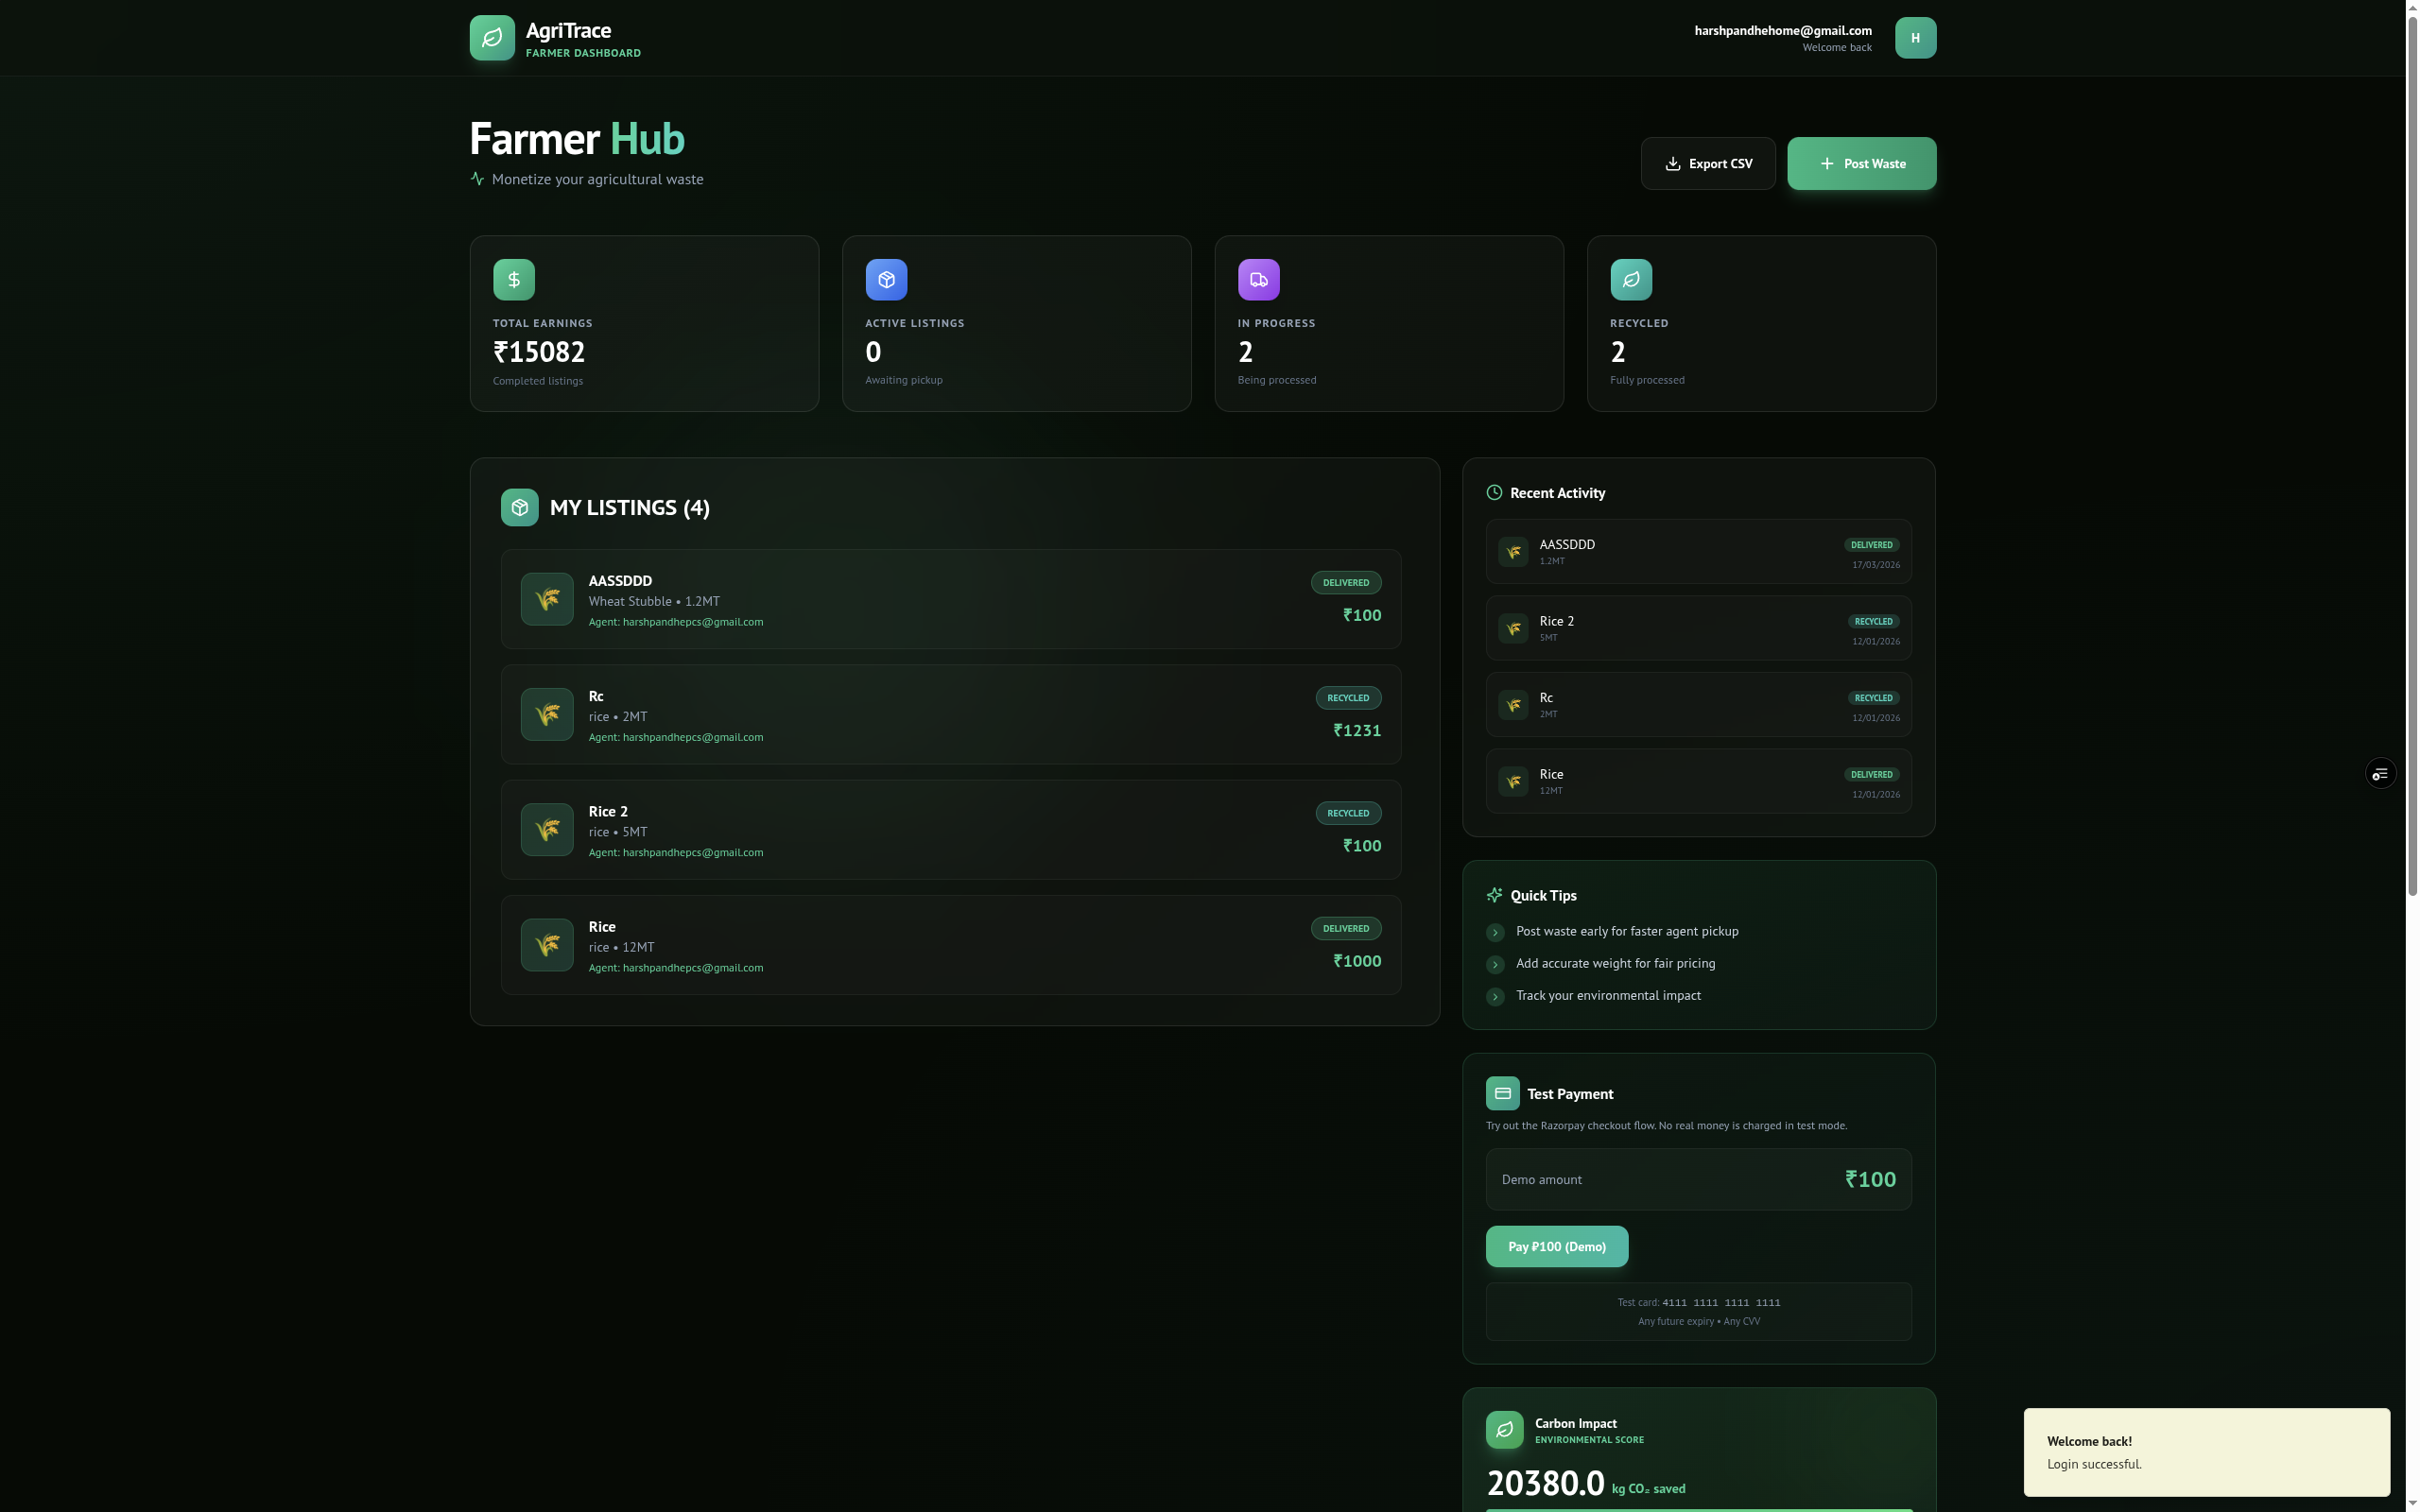
\includegraphics[width=0.9\textwidth]{images/output-farmer-new.png}
\caption{Farmer Dashboard detailing active waste listings and carbon offset accumulations.}
\label{fig:farmer}
\end{figure}

The seamless integration of Razorpay ensured that farmers securely received instant payment directly upon verified waste delivery updates by the agents, aggressively boosting platform trust. Furthermore, the localized Gamified Carbon Tracking component effectively visualized the environmental impact—logging equivalent metric CO2 savings derived actively from the sustainably diverted agricultural residue. 

\section{CONCLUSION}
AgriTrace demonstrates the immense viability of deploying a cohesive, digital ecosystem to aggressively tackle the monumental hurdle of agricultural residue burning. By deploying serverless architectures integrated with mobile-optimized frontends, the platform uniquely bridges the logistical disconnect between waste-generating farmers and recycling facilities. The platform inherently succeeds in curtailing severe atmospheric pollution while concurrently unlocking crucial secondary economic value from traditionally discarded biomass. Subsequent versions aim to deploy expansive multi-language support (Hindi, Marathi, Punjabi) enabling widespread adoption across diverse linguistic communities, coupled with IoT-assisted scale integrations to heavily automate collection weight verifications natively at pickup hubs.

\vspace{1em}
\noindent \textbf{ACKNOWLEDGEMENTS}\\
We would like to express our deepest gratitude to our project guide Mrs. S. A. GAIKWAD for her invaluable guidance, encouragement, and continuous support throughout this research work. We also extend our thanks to the faculty members of the Computer Engineering Department at S.P.M Polytechnic Kumathe for heavily bolstering our technical capabilities and guiding the platform's infrastructural development.

\section{REFERENCES}
[1] Next.js Official Documentation, Versel Inc., 2023. [Online]. Available: https://nextjs.org/docs\par
\vspace{0.5em}
[2] Firebase Realtime Database and Authentication, Google, 2023. [Online]. Available: https://firebase.google.com/docs\par
\vspace{0.5em}
[3] Ministry of Agriculture and Farmers Welfare, "National Policy for Management of Crop Residues," Government of India, 2014.\par
\vspace{0.5em}
[4] R. Kumar, S. Sharma, and A. Singh, "IoT-Based Monitoring of Agricultural Residue Burning," IEEE Sensors Journal, Vol. 20, No. 8, 2020, PP 4523-4531.\par
\vspace{0.5em}
[5] Central Pollution Control Board (CPCB), "Air Quality Monitoring Data," Government of India, 2023.\par

\end{document}
